\documentclass[12pt]{article}
\usepackage{tikz}

\begin{document}

\begin{center}
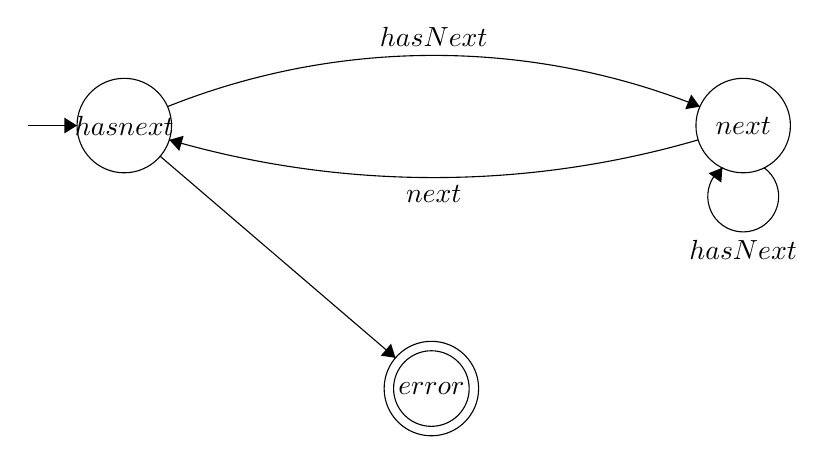
\begin{tikzpicture}[scale=0.2]
\tikzstyle{every node}+=[inner sep=0pt]
\draw [black] (35.4,-30.6) circle (3);
\draw (35.4,-30.6) node {$error$};
\draw [black] (35.4,-30.6) circle (2.4);
\draw [black] (15.9,-13.9) circle (3);
\draw (15.9,-13.9) node {$hasnext$};
\draw [black] (55.2,-13.9) circle (3);
\draw (55.2,-13.9) node {$next$};
\draw [black] (9.8,-13.9) -- (12.9,-13.9);
\fill [black] (12.9,-13.9) -- (12.1,-13.4) -- (12.1,-14.4);
\draw [black] (18.18,-15.85) -- (33.12,-28.65);
\fill [black] (33.12,-28.65) -- (32.84,-27.75) -- (32.19,-28.51);
\draw [black] (18.647,-12.696) arc (111.78302:68.21698:45.549);
\fill [black] (52.45,-12.7) -- (51.9,-11.93) -- (51.52,-12.86);
\draw (35.55,-8.94) node [above] {$hasNext$};
\draw [black] (52.342,-14.81) arc (-73.76829:-106.23171:60.073);
\fill [black] (18.76,-14.81) -- (19.39,-15.51) -- (19.67,-14.55);
\draw (35.55,-17.7) node [below] {$next$};
\draw [black] (56.523,-16.58) arc (54:-234:2.25);
\draw (55.2,-21.15) node [below] {$hasNext$};
\fill [black] (53.88,-16.58) -- (53,-16.93) -- (53.81,-17.52);
\end{tikzpicture}
\end{center}

\end{document}
